%% Programmatic weak supervision as masked-cause inference:
%% identifiability of label models without gold data.
%% Conference-format draft (target: 12 pages incl. references).

\documentclass[11pt,letterpaper]{article}

%% ============================================================================
%% Packages
%% ============================================================================

\usepackage{amsmath,amsthm,amssymb}
\usepackage{mathtools}
\usepackage{bm}
\usepackage{graphicx}
\graphicspath{{figures/}}
\usepackage{float}
\usepackage{booktabs}
\usepackage[shortlabels]{enumitem}
\usepackage[margin=1in]{geometry}
\usepackage{microtype}
\usepackage[colorlinks=true,linkcolor=blue,citecolor=blue,urlcolor=blue]{hyperref}
\usepackage{natbib}
\usepackage{cleveref}

%% Theorem environments
\theoremstyle{plain}
\newtheorem{theorem}{Theorem}
\newtheorem{proposition}[theorem]{Proposition}
\newtheorem{lemma}[theorem]{Lemma}
\newtheorem{corollary}[theorem]{Corollary}

\theoremstyle{definition}
\newtheorem{definition}[theorem]{Definition}
\newtheorem{condition}{Condition}
\crefname{condition}{Condition}{Conditions}
\Crefname{condition}{Condition}{Conditions}

\theoremstyle{remark}
\newtheorem{remark}[theorem]{Remark}

%% Macros
\newcommand{\E}{\mathbb{E}}
\newcommand{\Prob}{\mathbb{P}}
\newcommand{\R}{\mathbb{R}}
\newcommand{\1}{\mathbf{1}}
\newcommand{\X}{X}
\newcommand{\Y}{Y}

%% Title
\title{Programmatic weak supervision as masked-cause inference:\\
       identifiability of label models without gold data}

\author{
  Alexander Towell \\
  Department of Computer Science \\
  Southern Illinois University Edwardsville \\
  \texttt{lex@metafunctor.com} \\
  ORCID: \href{https://orcid.org/0000-0001-6443-9897}{0000-0001-6443-9897}
}

\date{\today}

\begin{document}

\maketitle

\begin{abstract}
Programmatic weak supervision trains classifiers from multiple noisy
labeling functions (LFs) instead of hand-labeled data. Frameworks
such as data programming and Snorkel fit a \emph{label model} that
aggregates LF votes into probabilistic training labels, ideally
without any gold-labeled examples. The central inferential question,
when the true labels can be recovered from LF votes alone, is a
masked-data identifiability problem from reliability statistics. We
make this precise: the true label is the latent cause, the set of
labels consistent with the LF votes is the candidate set, an LF
abstention is a non-informative (full) candidate set, a confident LF
vote is a narrowed candidate set, and a gold-labeled example is a
singleton candidate set that restores identifiability.

We establish: (i) a glass-ceiling theorem showing that without gold
labels and without a structural assumption on LF dependence, the LF
accuracies and class prior are non-identifiable, via an explicit
accuracy-complement symmetry construction; (ii) an identifiability
theorem recovering the Dawid--Skene, data-programming, and
triplet-method result as a masked-cause statement, under conditional
independence of LFs given the label; (iii) an agreement-consistency
theorem, the label-model analogue of cell-total consistency, showing
the fitted model reproduces empirical pairwise LF agreement rates
exactly at an interior MLE; and (iv) a gold-set sample-complexity
bound, $\Theta(r / \mathrm{gap}^2)$ for total (L2) model recovery in
the parameter-degeneracy dimension $r$ induced by LF dependence and
the accuracy margin, for restoring identifiability when LFs are
correlated.

A base-R simulation confirms each theorem; the dependent-case bound
is the load-bearing external contribution, and the empirical
$\log$--$\log$ slope of $-2.04$ for the gold-set size against the
accuracy margin matches the predicted $1/\mathrm{gap}^2$ factor (the
simulation isolates this gap factor; the linear-in-$r$ rate is proved
but not yet exercised by an $r$-sweep). The framework casts the
C1--C2--C3 coarsening conditions of
Heitjan--Rubin and Gill--van der Laan--Robins as a classification of
LF ensembles, and states, in coarsening-at-random terms, when a
gold-free weak-supervision pipeline is identifiable. Dawid--Skene
(1979) is the clear ancestor of label-model identifiability,
moment-based identifiability under conditional independence is
established prior work, and the candidate-subset view with gold-free
identifiability up to label swapping is due to Yu, Ding, and Bach
(2022); the contribution here is the masked-cause
unification, the C1--C2--C3 classification, the explicit
glass-ceiling construction, and the gold-set sample-complexity
theorem for the dependent case.
\end{abstract}

\section{Introduction}
\label{sec:intro}

Supervised learning needs labeled data, and hand-labeling is the
recurring bottleneck. Programmatic weak supervision attacks the
bottleneck by replacing hand-labels with \emph{labeling functions}
(LFs): small, noisy, user-written programs that vote on an example's
label or abstain \citep{ratner2016data,ratner2017snorkel}. A heuristic
keyword match, a regular expression, a knowledge-base lookup, or the
output of an off-the-shelf classifier each becomes one LF. Many LFs,
individually unreliable, collectively carry signal. The data
programming paradigm \citep{ratner2016data} and the Snorkel system
built on it \citep{ratner2017snorkel} fit a \emph{label model} that
estimates each LF's accuracy and aggregates the LF votes into
probabilistic training labels, which then train a downstream
classifier. The defining promise is gold-free supervision: no
hand-labeled examples are required to fit the label model.

That promise rests on an identifiability claim. The label model is
estimated from LF votes alone, so its parameters (per-LF accuracies,
the class prior) must be \emph{recoverable} from the distribution of
LF votes. When they are not, the fitted label model is one of many
that explain the votes equally well, and the probabilistic training
labels it emits are not trustworthy. The weak-supervision literature
has answered this question in pieces. \citet{dawid1979maximum}
established maximum-likelihood estimation of rater error rates by EM
in the crowdsourcing setting. \citet{ratner2016data} and the triplet
method of \citet{fu2020fast} proved that LF accuracies are
identifiable from agreement moments when the LFs are conditionally
independent given the label. \citet{ratner2019training} extended the
moment approach to structured dependence with a known dependency
graph. Closest to the present setting, \citet{yu2022nplm} let LFs emit
\emph{subsets} of candidate labels, fit a gold-free generative label
model over those subsets, and prove it is identifiable up to label
swapping under mild conditions; our work recovers their candidate-set
view and their label-swap obstruction (our \cref{sec:translation} and
\cref{thm:glass-ceiling}) as the weak-supervision instance of the
reliability-theoretic coarsening framework, and adds the
dependent-case gold-set sample-complexity analysis they do not treat.
What this body of work has not assembled is a single inferential frame
that classifies \emph{which} LF ensembles are identifiable, names the
auxiliary information that rescues the rest, and prices it.

\subsection{The bridge to masked-cause inference}

We observe that label-model estimation is an instance of the
masked-cause series-system identifiability problem from reliability
statistics \citep{towell2026masked}. In that framework, $m$
components in series produce a system that fails when any one fails;
the failed component is masked, but a \emph{candidate set} containing
it is observed. Identifiability of component-level parameters hinges
on coarsening-at-random conditions, the C1--C2--C3 conditions of
\citet{heitjan1991ignorability} and \citet{gill1997coarsening}, and a
\emph{singleton} candidate set (an observation where the cause is
known exactly) restores identifiability when broader coarsening is
confounded.

The translation to weak supervision is direct. The true label $Y$ is
the latent cause. The set of labels consistent with the LF votes for
an example is the candidate set. An LF that abstains contributes
nothing and leaves the candidate set full (a non-informative
coarsening); an LF that votes confidently narrows the candidate set;
a gold-labeled (hand-annotated) example pins the candidate set to a
singleton. The C1--C2--C3 conditions become a classification of LF
ensembles, and the masked-cause identifiability theorems give the
precise conditions under which a gold-free pipeline is identifiable.
The present paper is one application of the masked-cause framework
of \citet{towell2026masked}.\footnote{Sibling applications in the
framework series address scRNA-seq zero inflation, spatial
transcriptomics, differential privacy, and EHR phenotyping
\citep{towell2026scrnacoarsening,towell2026spatialcoarsening,
towell2026dpcoarsening,towell2026phenotypecoarsening}.}

\subsection{Contributions}

We contribute:

\begin{itemize}
\item \textbf{A bridge from programmatic weak supervision to
  masked-cause inference} (\cref{sec:translation}), expressing the
  label model of data programming and Snorkel as a coarsening problem
  and casting the C1--C2--C3 conditions as a classification of LF
  ensembles.

\item \textbf{A glass-ceiling theorem} (T1, \cref{sec:identifiability}):
  without gold labels and without a structural assumption on LF
  dependence, the LF accuracies and class prior are non-identifiable.
  We exhibit the obstruction explicitly as an accuracy-complement
  symmetry, broken only by an assumption such as ``LFs are better than
  random'' or conditional independence.

\item \textbf{An identifiability theorem under conditional
  independence} (T2, \cref{sec:identifiability}): with conditionally
  independent LFs and at least three of non-degenerate accuracy, the
  LF accuracies and class prior are identifiable from the second- and
  third-order agreement moments. This re-derives the
  Dawid--Skene / data-programming / triplet-method result as a
  masked-cause theorem.

\item \textbf{An agreement-consistency theorem} (T3,
  \cref{sec:identifiability}): the fitted label model reproduces the
  empirical pairwise LF agreement rates exactly at an interior MLE.
  This is the label-model analogue of the cell-total consistency
  result of \citet{towell2026scrnacoarsening}.

\item \textbf{A gold-set sample-complexity theorem} (T4,
  \cref{sec:methodology}): when LFs violate conditional independence,
  with the dependence inducing a parameter-degeneracy dimension $r$ in
  the agreement structure, the number of gold-labeled examples needed
  to restore the label model to total (L2) accuracy is
  $\Theta(r / \mathrm{gap}^2)$ in that degeneracy dimension and the
  accuracy margin, with matching upper and minimax lower bounds; the
  rate is loss-dependent, falling to $\Theta(\log r / \mathrm{gap}^2)$
  under a per-direction criterion. Singletons restore the rank that LF
  dependence destroys.

\item \textbf{Simulation validation} (\cref{sec:validation}). A
  base-R study confirms the glass-ceiling symmetry, gold-free recovery
  under conditional independence, agreement consistency to numerical
  precision, and the gold-set scaling under injected LF dependence.
\end{itemize}

The paper's message: gold-free weak supervision is not magic, it is a
coarsening problem with a precise identifiability boundary. The
C1--C2--C3 conditions tell a practitioner whether their LF ensemble
is on the identifiable side of that boundary, and the
sample-complexity theorem tells them how much gold data buys back
identifiability when it is not.

\section{Masked-cause inference: brief primer}
\label{sec:background}

We summarize the masked-cause identifiability framework
\citep{towell2026masked,heitjan1991ignorability,gill1997coarsening}.
Readers familiar with that work, or with the companion applications
\citep{towell2026scrnacoarsening,towell2026spatialcoarsening}, can
skim to \cref{sec:translation}.

Consider $m$ independent components in series. Each component $j$ has
a parametric distribution $f_j(\cdot;\theta_j)$ for its lifetime
$T_{ij}$ in system $i$. The system fails at $T_i = \min_j T_{ij}$
with cause $K_i = \arg\min_j T_{ij}$. We observe $T_i$ but not $K_i$
directly; instead we observe a \emph{candidate set} $C_i \subseteq
\{1,\ldots,m\}$ thought to contain the failed component.

The joint likelihood factorizes as
\begin{equation}
  f(t, k, c; \theta)
  = h_k(t; \theta_k) \prod_{\ell} R_\ell(t; \theta_\ell)
    \cdot \Prob_\theta\{C_i = c \mid T_i = t, K_i = k\},
  \label{eq:bg-joint}
\end{equation}
where $h_\ell$ is the component-$\ell$ hazard and $R_\ell$ its
survival function. The third factor is the unknown coarsening (or
masking) mechanism.

Three coarsening-at-random conditions allow the masking factor to
drop from the score:

\begin{condition}[Support, C1]
\label{cond:c1}
$\Prob\{K_i \in C_i\} = 1$: the true cause lies in the candidate set.
\end{condition}

\begin{condition}[Symmetry, C2]
\label{cond:c2}
$\Prob_\theta\{C_i=c \mid T_i=t, K_i=j\} = \Prob_\theta\{C_i=c \mid
T_i=t, K_i=k\}$ for all $j,k \in c$: the coarsening does not depend on
which element of the candidate set is the true cause.
\end{condition}

\begin{condition}[Parameter independence, C3]
\label{cond:c3}
$\Prob_\theta\{C_i=c \mid T_i, K_i\}$ does not depend on $\theta$: the
coarsening parameters are distinct from the component parameters.
\end{condition}

Under all three, the likelihood collapses to
\begin{equation}
  L_i(\theta) \propto \left[\prod_\ell R_\ell(t_i;\theta_\ell)\right]
  \cdot \left[\sum_{j \in c_i} h_j(t_i; \theta_j)\right],
  \label{eq:bg-c1c2c3}
\end{equation}
that is, the coarsening mechanism becomes ignorable for likelihood
inference.

\citet[Theorem 8]{towell2026masked} establish identifiability under
these conditions:

\begin{theorem}[Identifiability under C1--C2--C3]
\label{thm:bg-id}
Under \cref{cond:c1,cond:c2,cond:c3} and standard regularity
(in particular, positive probability assigned to both exact-event
and censored-type observations), full column rank $m$ of the
augmented candidate-set matrix $\tilde{C} \in \{0,1\}^{n \times m}$
is \emph{sufficient} for $\theta$ to be identifiable. Separability
is necessary but not in general sufficient (a separating mechanism
can leave $\tilde{C}$ rank-deficient, e.g. $m=4$ with candidate
sets $\{1,2\},\{3,4\},\{1,3\},\{2,4\}$).
\end{theorem}

\emph{Singleton} candidate sets ($|c_i|=1$) are the critical
ingredient: each isolates a single component contribution in
\eqref{eq:bg-c1c2c3} and adds an identifying unit-vector row to
$\tilde{C}$. When broader candidate sets are confounded (the matrix
$\tilde{C}$ is rank-deficient), singletons restore the missing rank.

This framework has been ported to single-cell RNA sequencing zero
inflation \citep{towell2026scrnacoarsening} and to
spatial-transcriptomics deconvolution
\citep{towell2026spatialcoarsening}. We now port it to programmatic
weak supervision. The candidate-set structure here is combinatorial:
each labeling function emits a vote (or abstains), and the
intersection of the votes defines the candidate set over labels. The
coarsening mechanism is the joint LF noise model, and the three
conditions become statements about how LF errors relate to the true
label and to the label-model parameters.

\section{Translation: the label model as a coarsening problem}
\label{sec:translation}

\subsection{The data-generating process}

Consider a binary classification task with true label $Y \in \{0,1\}$
and class prior $\pi = \Prob\{Y = 1\}$; the multiclass case is a
direct extension. There are $m$ labeling functions. For example $i$,
LF $j$ emits a vote $\lambda_{ij} \in \{0, 1, \varnothing\}$, where
$\varnothing$ denotes \emph{abstention}. Each LF $j$ has a
\emph{coverage} $\beta_j = \Prob\{\lambda_{ij} \neq \varnothing\}$,
the probability it does not abstain, and an \emph{accuracy}
$\alpha_j = \Prob\{\lambda_{ij} = Y \mid \lambda_{ij} \neq
\varnothing\}$, the probability it votes correctly given that it
votes. When LF $j$ votes, it emits $Y$ with probability $\alpha_j$
and the complementary label $1 - Y$ with probability $1 - \alpha_j$.

The label model is fit to the matrix of votes $\{\lambda_{ij}\}$. Its
parameters are the per-LF accuracies $\bm{\alpha} = (\alpha_1, \ldots,
\alpha_m)$, the coverages $\bm{\beta}$, and the class prior $\pi$.
Coverages are directly observed (each is an empirical abstention
rate), so the inferential content is the recovery of $\bm{\alpha}$
and $\pi$, after which the posterior $\Prob\{Y = y \mid
\bm{\lambda}_i\}$ supplies the probabilistic training label for
example $i$.

\subsection{LF votes as a candidate set}

The votes of the $m$ LFs on example $i$ induce a \emph{candidate set}
$c_i \subseteq \{0, 1\}$: the set of labels still consistent with the
observed votes under the modeled noise. An LF that abstains
constrains nothing. An LF that votes is consistent with both labels
(it could be voting correctly or incorrectly) until its accuracy is
known, but its vote shifts the posterior mass. In the deterministic
limit, where an LF that votes is treated as ground truth, a single
confident vote collapses the candidate set to that label; a
gold-labeled example fixes the candidate set to the singleton
$\{Y_i\}$ by construction. The probabilistic label model is the
soft-coarsening relaxation of this combinatorial picture: instead of
a hard candidate set, each example carries a distribution over
$\{0,1\}$ determined by the LF votes and the accuracy parameters.

This candidate-set reading of weak supervision is itself the subject
of an established line of work, which we connect to rather than
introduce. \citet{yu2022nplm} make LFs emit candidate-label subsets
explicitly and aggregate them with a gold-free generative model; the
partial-label and superset-label learning literatures study learning
a classifier when each example carries a candidate set known to
contain the truth, with the learnability boundary controlled by an
\emph{ambiguity degree} \citep{cour2011partial}, sample-complexity
conditions for empirical-risk minimization on supersets
\citep{liu2014superset}, consistent disambiguation losses with proved
rates \citep{cabannes2020infimum}, and a mixing-matrix admissibility
condition for proper losses on partial labels
\citep{cidsueiro2012proper}. Those works fix the candidate set as
given supervision and study how to learn from it; we instead treat the
candidate set as the \emph{output} of a coarsening mechanism whose
own parameters (LF accuracies, prior) must be identified, and read
the C1--C2--C3 conditions as the admissibility statement on that
mechanism.

\subsection{The translation}

\Cref{tab:translation} states the explicit correspondence to
masked-cause inference.

\begin{table}[ht]
\centering
\small
\begin{tabular}{@{}p{0.40\linewidth} p{0.56\linewidth}@{}}
\toprule
\textbf{Masked-data framework} & \textbf{Programmatic weak supervision} \\
\midrule
Component / latent cause $K_i$ & True label $Y$ \\
Candidate set $c_i$ & Labels consistent with the LF votes for an example \\
Masking probability & The per-LF accuracy / confusion model \\
Singleton candidate set $|c_i|=1$ & A gold-labeled (hand-annotated) example \\
Non-informative (full) candidate set & An LF that abstains \\
Narrowed candidate set & A confident LF vote \\
Augmented candidate-set matrix $\tilde C$ & The matrix of LF votes
  augmented with any gold labels; full column rank gives
  identifiability \\
C1 (truth in candidate set) & True label consistent with the votes;
  holds unless LFs are confidently wrong beyond modeled noise \\
\textbf{C2} (coarsening at random): conditional on the candidate set, the masking distribution does not depend on which element is the true cause &
  Concretely: LF error depends on $Y$ only through the modeled
  confusion, not on the label-model parameters \\
C3 (parameter independence) & LF accuracy parameters distinct from
  the downstream model parameters \\
\bottomrule
\end{tabular}
\caption{Translation between the masked-cause framework
\citep{towell2026masked} and programmatic weak supervision.}
\label{tab:translation}
\end{table}

The three conditions deserve a reading in the weak-supervision
language.

\paragraph{C1, support.} The true label must remain consistent with
the LF votes. This fails exactly when an LF is confidently wrong in a
way the noise model does not allow, for example an LF whose error is
systematic on a subpopulation (a label-conditional bias the
symmetric accuracy parameter cannot represent). For ordinary noisy
LFs, C1 holds: the modeled noise already admits any vote pattern.

\paragraph{C2, symmetry.} LF error must depend on $Y$ only through
the modeled confusion. An LF whose error rate is itself a function of
the label-model parameters, or whose mistakes are correlated with the
quantity being estimated, breaks C2. The standard data-programming
accuracy model satisfies C2 by construction: $\Prob\{\lambda_{ij}
\mid Y\}$ is a fixed confusion table.

\paragraph{C3, parameter independence.} The LF accuracy parameters
$\bm{\alpha}$ must be distinct from the downstream classifier's
parameters. This holds in the standard pipeline, where the label
model is fit first and the downstream model second; it would fail in
a joint end-to-end scheme that ties LF reliability to downstream
performance.

\subsection{Existing methods in this language}

\paragraph{Dawid--Skene \citep{dawid1979maximum}} fit per-rater
confusion matrices and a class prior by EM. In our language: the
candidate-set coarsening is the confusion table, and EM is the
maximum-likelihood solver for the coarsened likelihood
\eqref{eq:bg-c1c2c3}. Dawid--Skene is the clear ancestor of the
label model.

\paragraph{Data programming \citep{ratner2016data}} fits a
factor-graph label model and, in the independent case, recovers LF
accuracies from agreement statistics. This is identifiability under
C1--C2--C3 with conditionally independent LFs (\cref{sec:identifiability}).

\paragraph{Snorkel \citep{ratner2017snorkel}} is the system built on
data programming; the multi-task extension \citep{ratner2019training}
handles structured LF dependence with a known dependency graph. In
our language, a known dependency graph is a structural assumption
that repairs the rank deficit C2 violations would otherwise cause.

\paragraph{Triplet method \citep{fu2020fast}} recovers LF accuracies
in closed form from third-order agreement rates of conditionally
independent LFs. This is the constructive proof of T2 below.

\paragraph{Crowdsourcing \citep{karger2011iterative}} solves the same
estimation problem with workers in place of LFs and message-passing
in place of EM. The masked-cause frame covers both: a worker and an
LF are both noisy coarsenings of the true label.

These methods are not in conflict; they are different solvers and
parametrizations of one coarsening problem. The framework states
precisely when each is identifiable and what auxiliary information
(gold labels, a dependency graph, a better-than-random assumption)
each implicitly requires.

\section{Identifiability and agreement consistency}
\label{sec:identifiability}

We port \cref{thm:bg-id} to the label model. Three results follow:
the glass ceiling (T1), identifiability under conditional
independence (T2), and agreement consistency (T3).

\subsection{The glass ceiling: gold-free non-identifiability}

The label model is fit from LF votes alone. Whether its parameters
can be recovered from the vote distribution is an identifiability
question, and the answer without further structure is negative.

\begin{theorem}[Glass ceiling, gold-free non-identifiability]
\label{thm:glass-ceiling}
Let $\bm{\lambda}_i$ be the LF votes under the DGP of
\cref{sec:translation}, with unknown accuracies $\bm{\alpha}$,
coverages $\bm{\beta}$, and class prior $\pi$. Without gold-labeled
examples, and absent a structural assumption on LF dependence or LF
orientation, the pair $(\bm{\alpha}, \pi)$ is non-identifiable from
the distribution of LF votes: there exist distinct parameter sets
producing identical vote distributions. In particular the
accuracy-complement symmetry holds: replacing $(\pi, \bm{\alpha})$ by
$(1 - \pi,\ \1 - \bm{\alpha})$ leaves every joint vote probability
unchanged.
\end{theorem}

\begin{proof}[Sketch]
We exhibit non-identifiability by construction. Fix any example with
votes $\bm{\lambda}$. Under the symmetric accuracy model, the joint
probability of the votes marginalizing over $Y$ is
\begin{equation}
  \Prob\{\bm{\lambda}\}
  = \sum_{y \in \{0,1\}} \Prob\{Y = y\}
    \prod_{j:\,\lambda_j \neq \varnothing}
    \beta_j\, \alpha_j^{\1\{\lambda_j = y\}}
    (1-\alpha_j)^{\1\{\lambda_j \neq y\}}
    \prod_{j:\,\lambda_j = \varnothing} (1 - \beta_j).
  \label{eq:id-jointvote}
\end{equation}
Apply the relabeling $y \mapsto 1 - y$ inside the sum. The prior term
$\Prob\{Y = y\}$ becomes $\Prob\{Y = 1 - y\}$, which is the prior of
the parameter set with $\pi$ replaced by $1 - \pi$. Each factor
$\alpha_j^{\1\{\lambda_j = y\}}(1-\alpha_j)^{\1\{\lambda_j \neq y\}}$
becomes $\alpha_j^{\1\{\lambda_j \neq y\}}(1-\alpha_j)^{\1\{\lambda_j
= y\}}$, which is the factor of the parameter set with $\alpha_j$
replaced by $1 - \alpha_j$. The coverage factors are untouched. Hence
$(\pi, \bm{\alpha})$ and $(1 - \pi, \1 - \bm{\alpha})$ produce
identical $\Prob\{\bm{\lambda}\}$ for every vote pattern, so they are
observationally indistinguishable. An LF of accuracy $\alpha_j > 1/2$
is statistically a mirror image of one with accuracy $1 - \alpha_j <
1/2$ that has its output label flipped. The two solutions are
separated only by an external assumption: ``every LF is better than
random'' ($\alpha_j > 1/2$, fixing each LF's orientation), a fixed
class prior, or conditional independence with a known sign on one
agreement moment. The binary case exhibits the $\mathbb{Z}/2$
label-permutation element of the symmetric group; the multiclass
analog is the full symmetric group $\mathfrak{S}_K$ acting on
$\{0, 1, \ldots, K-1\}$, and the corresponding obstruction is
non-identifiability up to a label permutation. The reduction of the
gold-free obstruction to a rank condition on the augmented
candidate-set matrix is \cref{thm:bg-id} of \cref{sec:background};
the full apparatus, including regularity conditions, is in
\citet{towell2026masked}.
\end{proof}

\Cref{thm:glass-ceiling} is the weak-supervision instance of the
glass-ceiling phenomenon: an estimator that uses only LF votes cannot
orient the label model. It is the same structural obstruction that
\citet{towell2026scrnacoarsening} identify for scRNA-seq zeros, here
made fully explicit as a label-flip symmetry. The same obstruction
appears in the partial-labeler model of \citet{yu2022nplm}, who prove
gold-free identifiability only up to label swapping; \cref{eq:id-jointvote}
exhibits the binary witness of that swap symmetry in closed form and
ties the residual ambiguity to a rank deficit of the augmented
candidate-set matrix rather than leaving it as a generic permutation
caveat. A single gold-labeled example breaks the symmetry: it is a
singleton candidate set whose known label fixes the orientation,
adding an identifying row to the augmented candidate-set matrix of
\cref{thm:bg-id}. The
better-than-random assumption is the cost-free alternative when it is
credible; the next theorem shows what conditional independence buys
without any gold data.

\subsection{Identifiability under conditional independence}

The standard rescue in data programming is the assumption that LFs
err independently given the label. Under that assumption the label
model is identifiable from agreement moments alone.

\begin{theorem}[Identifiability under conditional independence]
\label{thm:ci-identifiability}
Suppose the LF votes are conditionally independent given $Y$, that at
least three LFs have non-degenerate accuracy ($\alpha_j \neq 1/2$ and
$0 < \beta_j \le 1$), and that LF orientations are fixed (e.g., every
LF is better than random). Then the accuracies $\bm{\alpha}$ and the
class prior $\pi$ are identifiable from the second- and third-order
LF agreement moments.
\end{theorem}

\begin{proof}[Sketch]
Encode each non-abstaining vote as $\sigma_{ij} = 2\,\1\{\lambda_{ij}
= 1\} - 1 \in \{-1, +1\}$ and the latent label as $Z = 2Y - 1$.
Conditional independence gives, for distinct LFs $j, k, \ell$ that
all vote,
\begin{equation}
  \E[\sigma_j \sigma_k] = a_j a_k, \qquad
  \E[\sigma_j \sigma_k \sigma_\ell] = a_j a_k a_\ell,
  \label{eq:id-triplet}
\end{equation}
where $a_j = \E[\sigma_j Z] = 2\alpha_j - 1$ is the LF's
\emph{accuracy margin} (its centered accuracy). Equation
\eqref{eq:id-triplet} is the moment structure exploited by the
triplet method of \citet{fu2020fast}. From three LFs, the three
pairwise products and the one triple product give
\begin{equation}
  a_j^2 = \frac{\E[\sigma_j \sigma_k]\,\E[\sigma_j \sigma_\ell]}
               {\E[\sigma_k \sigma_\ell]},
  \label{eq:id-solve}
\end{equation}
and symmetric expressions for $a_k, a_\ell$; the triple product fixes
the common sign, and the fixed-orientation assumption (or the
better-than-random assumption) selects $a_j > 0$. Each $a_j$
determines $\alpha_j = (1 + a_j)/2$. With the margins known, the
first moment $\E[\sigma_j] = a_j\,\E[Z] = a_j(2\pi - 1)$ identifies
$\pi$. Non-degeneracy ($a_j \neq 0$) keeps every denominator nonzero.
This is the data-programming and Dawid--Skene identifiability result
\citep{dawid1979maximum,ratner2016data,fu2020fast} re-derived as a
masked-cause statement: conditional independence makes the augmented
candidate-set matrix full column rank, so \cref{thm:bg-id} applies
and $(\bm{\alpha}, \pi)$ is identifiable without gold data.
\end{proof}

\Cref{thm:ci-identifiability} is the positive counterpart of T1.
Conditional independence is the structural assumption that breaks the
glass ceiling without gold labels: it supplies the moment equations
\eqref{eq:id-triplet} whose rank is exactly the augmented
candidate-set rank of \cref{thm:bg-id}. The fixed-orientation
assumption (each LF is declared to vote on the positive side of its
target class) is a checkable property of each LF's source code; it
is not automatic, however, since an LF written backward (a regex
that positively matches the negative class) reverses its sign and
silently violates the assumption. The assumption is also the
fragile one. When LFs share error structure (two regex LFs keyed on
the same token, two model-based LFs sharing a backbone), the products
in \eqref{eq:id-triplet} pick up cross terms, the rank drops, and the
gold-free estimator is biased. \Cref{sec:methodology} quantifies how
much gold data restores the lost rank.

\subsection{Agreement consistency}

A structural property holds for any label model fit by maximum
likelihood, regardless of whether the conditional-independence
assumption is correct: the fitted model reproduces the empirical
pairwise LF agreement rates.

\begin{theorem}[Agreement consistency, regular exponential family]
\label{thm:agreement-consistency}
Let $(\hat{\bm{\alpha}}, \hat{\pi})$ be a maximum-likelihood estimate
of the label model for a parametrization that forms a regular
exponential family whose sufficient statistics include the pairwise
LF agreement indicators $\1\{\lambda_{ij} = \lambda_{ik}\}$ (the
standard naive-Bayes parametrization of \citet{ratner2016data} does
not satisfy this hypothesis exactly; an asymptotic version of the
identity for the naive-Bayes corner is given in
\cref{cor:agreement-nb} below). Then for
every pair of LFs $(j, k)$,
\begin{equation}
  \widehat{\Prob}\{\lambda_j = \lambda_k \mid \text{both vote}\}
  = \bar{A}_{jk},
  \label{eq:agreement}
\end{equation}
where $\bar{A}_{jk}$ is the empirical agreement rate of LFs $j$ and
$k$ on the examples where both vote. The identity holds exactly at
any \emph{interior} MLE (no $\hat\alpha_j \in \{0,1\}$, no
$\hat\beta_j \in \{0,1\}$, $\hat\pi \in (0,1)$); boundary cases
reduce to degenerate-LF identities.
\end{theorem}

\begin{proof}[Sketch]
The argument parallels the cell-total consistency proof of
\citet[\S 3]{towell2026scrnacoarsening}. For a regular exponential
family the MLE satisfies the moment-matching identity
$\E_{\hat\theta}[T(\bm{\lambda})] = \bar{T}$ for every sufficient
statistic $T$ (the stationarity of the log-partition gradient). When
$T$ is the pair-$(j,k)$ agreement indicator
$\1\{\lambda_{ij} = \lambda_{ik}\}$ this is exactly
\eqref{eq:agreement}. The full derivation, including the boundary
regimes, is the moment-matching argument of
\citet{towell2026scrnacoarsening} with the candidate-set sufficient
statistic specialized to LF agreement.
\end{proof}

The conditioning matters: the identity \eqref{eq:agreement} is a
sufficient-statistic consequence, so it follows whenever the
parametrization is rich enough to count pairwise agreement among its
sufficient statistics. The standard naive-Bayes label model of data
programming \citep{ratner2016data} parametrizes by per-LF accuracies
$\bm{\alpha}$ and the class prior $\pi$; the pairwise agreement
indicators are \emph{not} per-pair sufficient statistics of that
parametrization. The result still applies in a weaker, asymptotic
sense for the conditionally independent corner:

\begin{corollary}[Asymptotic agreement consistency for naive-Bayes]
\label{cor:agreement-nb}
Under the conditional-independence assumption of
\cref{thm:ci-identifiability}, the naive-Bayes label model
parametrized by $(\bm{\alpha}, \pi)$ satisfies
\eqref{eq:agreement} asymptotically: at the population
parameter values the joint vote factorization implies $\Prob\{
\lambda_j = \lambda_k\} = \alpha_j \alpha_k + (1-\alpha_j)(1-\alpha_k)$
exactly, and the MLE converges to that value at the standard
$n^{-1/2}$ rate. The identity holds in the limit, not at every finite
sample.
\end{corollary}

The simulation in \cref{sec:validation} confirms this asymptotic
behavior at large $n$: the agreement residual decays as $n^{-1/2}$
and reaches Monte-Carlo noise at $n = 500{,}000$. The simulation is
consistent with \cref{thm:agreement-consistency} for the extended
exponential-family parametrization and with \cref{cor:agreement-nb}
for the naive-Bayes parametrization; it does not isolate the
sufficient-statistic property structurally.

\Cref{thm:agreement-consistency} is the label-model analogue of
cell-total consistency. Its practical force is a warning. Two label
models, one assuming conditional independence and one fit with a
dependency graph, can both reproduce every observed pairwise
agreement rate exactly (the first via \cref{cor:agreement-nb}
asymptotically, the second via \cref{thm:agreement-consistency} at
the exact MLE), while disagreeing on the LF accuracies and hence on
the probabilistic training labels. A practitioner checking ``does
the fitted model match the observed LF agreement?'' will see a
perfect fit from a biased model. Diagnosing accuracy bias requires
either gold labels or an external structural assumption; the marginal
agreement fit cannot do it. The same caution was raised for the ZINB
MLE in \citet{towell2026scrnacoarsening}; here it is sharper, because
the dependent and independent label models satisfy
\eqref{eq:agreement} jointly yet imply different supervision.
Agreement consistency (\cref{thm:agreement-consistency}) is a special
case of the general coarsened-data consistency theorem of
\citet{towell2026synthesis}, in which the singleton-candidate-set
device used here, gold labels, appears as one instance of a
domain-independent rank condition and singleton-restoration mechanism.

\section{Gold-set sample complexity under LF dependence}
\label{sec:methodology}

The identifiability theorem T2 (\cref{thm:ci-identifiability}) rests
on conditional independence of the LFs. In practice LFs are
correlated: they share tokens, share knowledge bases, or share model
backbones. Correlated error breaks C2 (\cref{cond:c2}), the triplet
moments \eqref{eq:id-triplet} pick up cross terms, and the gold-free
label model is biased. This section quantifies the remedy. Gold
labels are singleton candidate sets; we ask how many are needed to
restore identifiability, and answer with a sample-complexity bound
governed by the rank deficit the dependence induces and the LF
accuracy margin.

\subsection{Setup}

Let $A \in \R^{m \times m}$ be the population matrix of centered
pairwise LF agreements, $A_{jk} = \E[\sigma_j \sigma_k]$ for $j \neq
k$. Under conditional independence (\cref{thm:ci-identifiability}),
the off-diagonal of $A$ is rank one: $A_{jk} = a_j a_k$, the outer
product $\bm{a}\bm{a}^\top$ of the accuracy-margin vector $\bm{a}$.
That rank-one structure is precisely what makes
\eqref{eq:id-solve} solvable from agreement moments alone.

LF dependence perturbs $A$. Suppose a set of LF pairs shares latent
noise, so that
\begin{equation}
  A = \bm{a}\bm{a}^\top + E,
  \label{eq:meth-decomp}
\end{equation}
where $E$ is the symmetric, zero-diagonal dependence-induced
correction. The quantity that governs the gold budget is not the rank
of $E$ but the \emph{parameter-degeneracy dimension}
\begin{equation}
  r \;=\; d_{\mathrm{free}},
  \label{eq:meth-dfree}
\end{equation}
the dimension of the affine family of margin vectors $\bm{a}$
consistent with the gold-free agreement moments when the dependence
support is unknown, equivalently the corank of the off-diagonal
moment-map Jacobian as the low-rank correction $E$ ranges over its
unknown support. For generic instances in the practical regime
$r \ll m$ this degeneracy dimension equals the number of dependent
directions of shared LF error: for pairwise dependence, $r$ is the
number of dependent LF pairs. With $r > 0$ the off-diagonal of $A$ is
no longer rank one, the triplet identities fail, and $(\bm{\alpha},
\pi)$ is not identifiable from LF votes alone. This is the label-model
analogue of a rank-deficient candidate-set matrix in \cref{thm:bg-id}:
the dependence has destroyed $r$ identifying directions.

\begin{remark}[The degeneracy dimension versus the residual-matrix rank]
\label{rmk:r-definition}
The parameter-degeneracy dimension $r = d_{\mathrm{free}}$ is the
object that sets the rate, and it is not the same as the rank of the
symmetric agreement-residual matrix $A - \hat{\bm{a}}\hat{\bm{a}}^\top$
reported by a rank-one-fit diagnostic. For $K$ disjoint dependent LF
pairs the residual matrix perturbs a symmetric $2 \times 2$ block per
pair and so has rank $2K$, while the parameter degeneracy that gold
must pin has dimension $K$. The residual-matrix rank is therefore
twice the parameter-degeneracy dimension under pairwise dependence,
$\mathrm{rank}(A - \hat{\bm{a}}\hat{\bm{a}}^\top) = 2 d_{\mathrm{free}}$;
a practitioner reading $r$ off the residual-matrix rank must halve it.
\end{remark}

Define the \emph{accuracy margin} (or gap) of the ensemble as
\begin{equation}
  \mathrm{gap} = \min_j |2\alpha_j - 1| = \min_j |a_j|,
  \label{eq:meth-gap}
\end{equation}
the smallest centered accuracy among the LFs. The gap measures how
far the weakest LF is from a coin flip; it controls the
signal-to-noise ratio of every agreement moment.

\subsection{The sample-complexity bound}

A gold-labeled example is a singleton candidate set: its label $Y_i$
is known, so it directly observes the LF errors on that example,
$\1\{\lambda_{ij} \neq Y_i\}$, for every LF that votes. A gold set of
size $n_g$ supplies $n_g$ identifying rows. The question is how large
$n_g$ must be to restore the $r$ directions that dependence destroyed.

\begin{theorem}[Gold-set sample complexity, total model recovery]
\label{thm:goldset}
Let the LF agreement structure satisfy \eqref{eq:meth-decomp} with
parameter-degeneracy dimension $r = d_{\mathrm{free}}$ as in
\eqref{eq:meth-dfree}, and let the ensemble have accuracy margin
$\mathrm{gap}$ as in \eqref{eq:meth-gap}. Suppose the gold-labeled
examples are drawn i.i.d.\ from the same distribution, and fix the
success criterion to be \emph{total model recovery in the Euclidean
(L2) margin error}: the hybrid agreement-moment-plus-gold estimator
$\hat{\bm{a}}$ should satisfy $\|\hat{\bm{a}} - \bm{a}\|_2 \le c_0\,
\mathrm{gap}$, equivalently it should keep the downstream training-label
posterior KL below a fixed budget (\cref{rmk:l2-loss}). Then there are
constants $c, C$, depending only on the LF coverages and on bounded
moments of the vote distribution, such that with
\begin{equation}
  n_g \;\ge\; \frac{C}{\mathrm{gap}^2}
        \cdot \bigl(r + \log\tfrac{1}{\delta}\bigr)
  \label{eq:goldset-bound}
\end{equation}
gold-labeled examples the label model $(\bm{\alpha}, \pi)$ is recovered
to total accuracy $\|\hat{\bm{a}} - \bm{a}\|_2 \le c_0\,\mathrm{gap}$
with probability at least $1 - \delta$, and this rate is minimax
optimal in $r$ and $\mathrm{gap}$:
\begin{equation}
  n_g \;=\; \Omega\!\left(\frac{r}{\mathrm{gap}^2}\right)
  \label{eq:goldset-lower}
\end{equation}
is necessary, so the gold-set sample complexity for total recovery is
$\Theta(r/\mathrm{gap}^2)$, linear in the degeneracy dimension.
Conversely, when $r = 0$ (conditionally independent LFs) no gold labels
are required, recovering \cref{thm:ci-identifiability}.
\end{theorem}

\begin{proof}[Sketch]
\emph{Gold is a full-vector diagonal measurement.} On a gold example
$i$ with known label $Y_i$, the centered correctness statistic
$\xi_{ij} = 2\cdot\1\{\lambda_{ij} = Y_i\} - 1 \in \{-1, +1\}$ has
$\E[\xi_{ij} \mid \text{votes}] = a_j$ and variance $1 - a_j^2$, since
$\1\{\lambda_{ij} = Y_i\}$ is Bernoulli$(\alpha_j)$ and $4
\alpha_j(1-\alpha_j) = 1 - (2\alpha_j - 1)^2$. The gold sample mean
$\bar{\bm{\xi}}$ is therefore an unbiased, sub-Gaussian estimate of the
\emph{whole} margin vector $\bm{a}$ with diagonal covariance
$\Sigma/n_g$, $\Sigma_{jj} = (1 - a_j^2)/\beta_j \le 1/\beta_{\min}$,
where $\beta_{\min} = \min_j \beta_j > 0$ is the minimum coverage. The
per-coordinate precision is set by the marginal accuracy alone and is
indifferent to the dependence among LFs (the dependence enters only the
off-diagonal of $\Sigma$).

\emph{Reduction to the $r$-dimensional location model.} The plentiful
unlabeled agreement moments fix $\bm{a}$ on the $(m-r)$-dimensional
identified subspace; what gold must supply is the component of $\bm{a}$
in the $r$-dimensional degenerate subspace $U = \mathrm{col}(B)$,
$B^\top B = I_r$ (\cref{rmk:r-definition}). Projecting the gold mean
onto $U$ leaves the $r$-dimensional sub-Gaussian location model:
estimate $\bm\theta = B^\top \bm{a}$ from $n_g$ observations with mean
$\bm\theta$ and covariance $(1/n_g)\, B^\top \Sigma B$, whose
eigenvalues lie in $[\,(1-\mathrm{gap}^2)/\beta_{\max},\,
1/\beta_{\min}\,] = \Theta(1)$. The relevant tolerance along $U$ is
$\Theta(\mathrm{gap})$: the degenerate directions are precisely the
ones the agreement moments leave open, and the competing solutions sit
at separation proportional to $\mathrm{gap}$ (a small gap makes the
near-degenerate solutions close, the same way a small singular value
makes a rank condition fragile in \cref{thm:bg-id}).

\emph{Upper bound (trace bound, linear in $r$).} Take $\hat{\bm{a}}$ to
be the agreement fit on the identified subspace plus the projection $B
B^\top \bar{\bm{\xi}}$ of the gold mean onto $U$. The agreement term
vanishes with the unlabeled corpus, and the gold term has expected
squared error
\begin{equation}
  \E\,\bigl\| B B^\top(\bar{\bm{\xi}} - \bm{a}) \bigr\|_2^2
   = \mathrm{trace}\!\bigl( (1/n_g)\, B^\top \Sigma B \bigr)
   \;\le\; \frac{r}{n_g\, \beta_{\min}}.
  \label{eq:trace-bound}
\end{equation}
The trace of the projected covariance is what makes the error
\emph{linear in $r$}: each of the $r$ degenerate coordinates
contributes $\Theta(1/n_g)$ to the total squared error. A sub-Gaussian
chi-square (Bernstein / Hanson--Wright) tail
\citep{wainwright2019high} sharpens the deviation to
$\|B^\top(\bar{\bm{\xi}} - \bm{a})\|_2^2 \le C(r + \log(1/\delta))/(n_g
\beta_{\min})$ with probability $1 - \delta$, so requiring this below
$(c_0\,\mathrm{gap})^2$ gives \eqref{eq:goldset-bound}. No $\log r$
factor appears: the trace bound targets the total L2 error directly,
not each direction separately.

\emph{Lower bound (Gaussian-location minimax).} Restricting to a
sub-family with $E$ in a fixed $r$-dimensional subspace and $\bm{a}$
ranging over the $r$-dimensional affine manifold embeds the
$r$-dimensional Gaussian location model with per-coordinate variance
$\ge c_0 = (1 - \mathrm{gap}^2)/\beta_{\max} > 0$ and $n_g$ samples
inside the problem, so its minimax risk lower-bounds the full risk. The
minimax L2 squared risk of the $r$-dimensional Gaussian location model
is $\inf_{\hat{\bm{a}}}\sup_{\bm{a}} \E\|\hat{\bm{a}} - \bm{a}\|_2^2 \ge
c_0\, r/n_g$ (the Bayes risk under an isotropic $N(0, \tau^2 I_r)$ prior
tends to $c_0 r/n_g$ as $\tau \to \infty$ and lower-bounds the minimax
risk; equivalently the Cram\'er--Rao bound with diagonal Fisher
information $n_g/c_0$ per coordinate, \citealp{vandervaart1998asymptotic}).
This is information-theoretic, hence binds every estimator, not just the
hybrid one. Forcing the supremum risk below $(c_0\,\mathrm{gap})^2$
requires $n_g \ge (c_0/c_0^2)\, r/\mathrm{gap}^2$, which is
\eqref{eq:goldset-lower}. Together with the upper bound the gold-set
sample complexity for total recovery is $\Theta(r/\mathrm{gap}^2)$.

The reduction of the degenerate directions to the corank of the
augmented moment map, and the regularity conditions on coverages and
moments, follow the apparatus of \citet[\S 7]{towell2026masked}; the
singleton-restores-rank step is the weak-supervision instance of the
corresponding spike-in and single-cell-resolution results of
\citet{towell2026scrnacoarsening,towell2026spatialcoarsening}.
\end{proof}

\begin{remark}[The L2 criterion is the operative one]
\label{rmk:l2-loss}
The success criterion in \cref{thm:goldset} is total L2 recovery
because that is the loss the downstream training labels actually
depend on. The naive-Bayes posterior log-odds is linear in $\bm{a}$,
$\mathrm{logit}\,\Prob\{Y = 1 \mid \bm\lambda\} = \mathrm{logit}\,\pi
+ \sum_{j\text{ votes}} s_j\, w(a_j)$ with $w(a) = \log\frac{1+a}{1-a}$,
so a margin perturbation $\bm{a} \to \bm{a} + d\bm{a}$ changes the
expected KL of the perturbed training-label posterior from the true one
by a positive-semidefinite quadratic form $d\bm{a}^\top G\, d\bm{a}$
that is a coverage-weighted sum over LFs. Label quality is thus governed
by the L2 (sum-of-squares) margin error and is invariant to how a fixed
$\|d\bm{a}\|_2$ budget is spread across LFs. ``Restore the label model
to fixed label quality'' is therefore the total/L2 criterion, and the
operative gold-set rate is the linear-in-$r$ rate
$\Theta(r/\mathrm{gap}^2)$ of \cref{thm:goldset}.
\end{remark}

\begin{remark}[The rate is loss-dependent: L2, $L_\infty$, and RMS]
\label{rmk:r-dependence}
The gold-set sample complexity differs by success criterion, and each
rate is tight for its own loss; they are rates for different losses, not
competing bounds on one quantity. For \emph{total} (L2) model recovery,
$\|\hat{\bm{a}} - \bm{a}\|_2 \le c_0\,\mathrm{gap}$, the rate is
$\Theta(r/\mathrm{gap}^2)$ (\cref{thm:goldset}): the trace bound
\eqref{eq:trace-bound} makes the error linear in $r$ and the Gaussian
location minimax bound \eqref{eq:goldset-lower} shows no estimator does
better. For \emph{per-direction} ($L_\infty$) control, requiring every
one of the $r$ degenerate directions below $c_1\,\mathrm{gap}$
simultaneously, a per-direction Hoeffding bound and a union over the $r$
directions give $2r\exp(-2 n_g \beta_{\min}(c_1\,\mathrm{gap})^2) \le
\delta$, i.e.\
\begin{equation}
  n_g \;\ge\; \frac{1}{2 c_1^2 \beta_{\min}}
        \cdot \frac{1}{\mathrm{gap}^2}\,\log\!\frac{2r}{\delta},
  \label{eq:goldset-linf}
\end{equation}
the $\Theta(\log r/\mathrm{gap}^2)$ rate; the matching lower bound is
the maximum of $r$ sub-Gaussian coordinates, $\sim \sqrt{2\log r}$, so
the union bound is tight for the $L_\infty$ loss rather than loose. For
\emph{per-coordinate} root-mean-square control, $\|\hat{\bm{a}} -
\bm{a}\|_2/\sqrt{r} \le c_0\,\mathrm{gap}$, the $r$ in the trace bound
cancels the $\sqrt{r}$ normalization and the rate is
$\Theta(1/\mathrm{gap}^2)$, independent of $r$. The volume heuristic
sometimes offered for the linear-$r$ rate (competing-solution volume
$\sim \mathrm{gap}^r$, per-direction resolution
$\mathrm{gap}/\sqrt{r}$, hence $n_g \sim r/\mathrm{gap}^2$) is exactly
the L2 calculation \eqref{eq:trace-bound} and is the correct
proof of the L2 rate, not a conjecture about a separate quantity.
\end{remark}

\begin{remark}[Marginal-preserving DGPs]
\label{rmk:marginal-dgps}
The Bernoulli step of the proof uses only the marginal accuracy
$\alpha_j$ of each LF, not the dependence structure that couples LF
errors. Any data-generating process that preserves the LF marginals
(e.g., a Gaussian-copula shared-noise construction, a logistic
shared-noise construction, or a direct $E$-matrix perturbation)
produces the same gold-augmented Bernoulli draws and so satisfies the
same bound \eqref{eq:goldset-bound} on $\mathrm{gap}$. The
dependence mechanism enters \emph{only} through the rank deficit $r$,
not through the gap factor.
\end{remark}

\subsection{Interpretation}

\Cref{thm:goldset} makes the gold-free promise of weak supervision
precise rather than absolute. Three regimes follow from
\eqref{eq:goldset-bound}.

\paragraph{Conditionally independent LFs ($r = 0$).} No gold labels
are needed. The agreement moments alone identify the model, as T2
states. This is the regime data programming was designed for.

\paragraph{Mildly dependent LFs (small $r$).} A modest gold set
suffices, and for total model recovery the requirement scales linearly
in the number $r$ of independent shared-error directions
(\cref{thm:goldset}): each degenerate direction adds a constant
$\Theta(1/\mathrm{gap}^2)$ of gold. (\Cref{rmk:r-dependence} records
that the weaker per-direction $L_\infty$ criterion scales only as
$\log r$, and the per-coordinate RMS criterion is independent of $r$;
the operative criterion for the training labels is the L2 one,
\cref{rmk:l2-loss}.)

\paragraph{Small accuracy margin (small $\mathrm{gap}$).} The gold
requirement scales as $1/\mathrm{gap}^2$. An ensemble of LFs that are
all close to random voting needs quadratically more gold data,
because the near-degenerate solutions T1 leaves open are then close
together and hard to separate. Strong, confident LFs are cheap to
identify; weak ones are expensive.

The bound is the operational form of ``singletons restore the rank
that coarsening destroys.'' LF dependence is the coarsening pathology;
gold-labeled examples are the singletons; the rank deficit $r$ and
the gap $\mathrm{gap}$ together set the price.

\paragraph{A budgeting procedure.} A practitioner can use
\eqref{eq:goldset-bound} as a four-step rule:
\begin{enumerate}[label=(\arabic*)]
\item \emph{Pilot fit.} Fit a gold-free label model (triplet method
  or EM) and read off pilot estimates $\hat{\bm{\alpha}}^{(0)}$ and
  $\hat\pi^{(0)}$.
\item \emph{Estimate the gap.} Set
  $\widehat{\mathrm{gap}} = \min_j |2\hat\alpha_j^{(0)} - 1|$.
\item \emph{Estimate the degeneracy dimension.} Compute the centered
  pairwise LF agreement matrix $\hat A$ and its best rank-one fit
  $\hat{\bm{a}}\hat{\bm{a}}^\top$, and count the singular values of the
  residual $\hat A - \hat{\bm{a}}\hat{\bm{a}}^\top$ above a noise floor.
  This count is the residual-matrix rank; by \cref{rmk:r-definition}
  the parameter-degeneracy dimension under pairwise dependence is
  \emph{half} of it, $\hat r = \tfrac{1}{2}\,\mathrm{rank}(\hat A -
  \hat{\bm{a}}\hat{\bm{a}}^\top)$, so halve the count before
  provisioning to avoid a factor-of-two overestimate.
\item \emph{Provision.} Use \eqref{eq:goldset-bound} with the
  plug-in $(\hat r, \widehat{\mathrm{gap}})$ to set the gold-set
  budget $n_g$, which is linear in $\hat r$ for total recovery.
\end{enumerate}

The genuinely new content relative to data programming and the
triplet method is this dependent-case budget: prior work establishes
the $r = 0$ corner, and the framework extends it to the correlated
ensembles that practice actually produces.

\section{Validation}
\label{sec:validation}

We validate the four theorems on simulated weak-supervision data with
known ground-truth labels and LF parameters. All results are
reproducible from \texttt{scripts/run.R} (seed \texttt{20260521}),
which sources the data-generating process and estimators in
\texttt{scripts/sim.R}; the study uses base R only.

\subsection{Data-generating process}

The true label $Y \in \{0,1\}$ is drawn with prior $\pi$. Each
labeling function $j$ has coverage $\beta_j$ (probability it does not
abstain) and accuracy $\alpha_j$ (probability it votes $Y$ given that
it votes). LF $j$ votes correctly iff a latent Gaussian score
$g_j$ falls below the $\alpha_j$ quantile, which fixes the marginal
correctness probability at $\alpha_j$ exactly. For conditionally
independent LFs the scores are independent. For a dependent pair the
two scores share a common latent factor with weight
$\rho = \mathrm{dep}$, so the pair's errors are positively
correlated while each LF keeps its marginal accuracy
(the construction is marginal-preserving). This
construction breaks the rank-one agreement structure that T2 relies
on without changing what a gold-labeled example observes. As
\cref{rmk:marginal-dgps} formalizes, the proof of \cref{thm:goldset}
uses only the marginal accuracy of each LF (the Bernoulli step in
the gold-augmented estimator), so any marginal-preserving dependence
mechanism, Gaussian copula, logistic shared noise, or direct
$E$-matrix perturbation, gives the same gap-dependence; the
empirical slope reported below confirms the bound for the
Gaussian-copula construction. Three
estimators are used: the gold-free label model (closed-form triplet
method of moments on pairwise and triple agreement rates, then the
naive-Bayes posterior $\Prob\{Y \mid \bm{\lambda}\}$); the
gold-augmented model (LF accuracies pinned directly from
$m_{\mathrm{gold}}$ gold-labeled examples); and the oracle (true
$Y$).

\subsection{Glass ceiling (\cref{thm:glass-ceiling})}

We generate five conditionally independent LFs ($\bm{\alpha} =
(0.85, 0.78, 0.72, 0.68, 0.90)$, coverage $0.7$, prior $\pi = 0.4$)
and enumerate all $3^5 = 243$ vote patterns over $\{0, 1,
\text{abstain}\}$. For each pattern we compute the probability under
the true parameter set, solution A $= (\pi, \bm{\alpha})$, and the
flipped set, solution B $= (1 - \pi, \1 - \bm{\alpha})$. The two
solutions produce identical pattern probabilities: the maximum
absolute difference $\max_{\bm{\lambda}} |\Prob_A\{\bm{\lambda}\} -
\Prob_B\{\bm{\lambda}\}|$ is $0$ to floating-point precision (not
small, exactly zero). Both solutions fit the empirical vote
distribution from $200{,}000$ examples equally well, each with $L_1$
distance $0.0257$ to the empirical distribution. The
accuracy-complement symmetry of \cref{thm:glass-ceiling} is therefore
exact: an estimator that uses only LF votes cannot orient the label
model. The gold-free triplet method recovers the unsigned margins
$|a_j|$ and, with the better-than-random orientation assumption
supplied, lands on solution A: estimated accuracies $(0.851, 0.777,
0.722, 0.682, 0.899)$ against the truth $(0.85, 0.78, 0.72, 0.68,
0.90)$, and $\hat\pi = 0.400$. Without that assumption solution B is
equally admissible.

\subsection{Identifiability under conditional independence
(\cref{thm:ci-identifiability})}

We generate five conditionally independent LFs ($\bm{\alpha} =
(0.82, 0.75, 0.70, 0.88, 0.66)$, mixed coverage, $\pi = 0.45$) and
sweep the number of examples $n$ over $\{500, \ldots, 50{,}000\}$,
$30$ replicates per setting. The gold-free triplet estimator recovers
the LF accuracies with median RMSE falling from $0.046$ at $n = 500$
to $0.0044$ at $n = 50{,}000$ (\Cref{fig:identifiability}A); the
log--log slope of RMSE against $n$ is $-0.53$, consistent with the
$n^{-1/2}$ rate of a method-of-moments estimator. The class prior is
recovered with median absolute error falling from $0.028$ to
$0.0025$ over the same range. True-label recovery accuracy from the
gold-free posterior reaches $0.871$, statistically indistinguishable
from the oracle ceiling of $0.872$ (\Cref{fig:identifiability}B). The
gold-free label model is identifiable under conditional independence
and converges to the oracle, as \cref{thm:ci-identifiability}
predicts.

\begin{figure}[t]
\centering
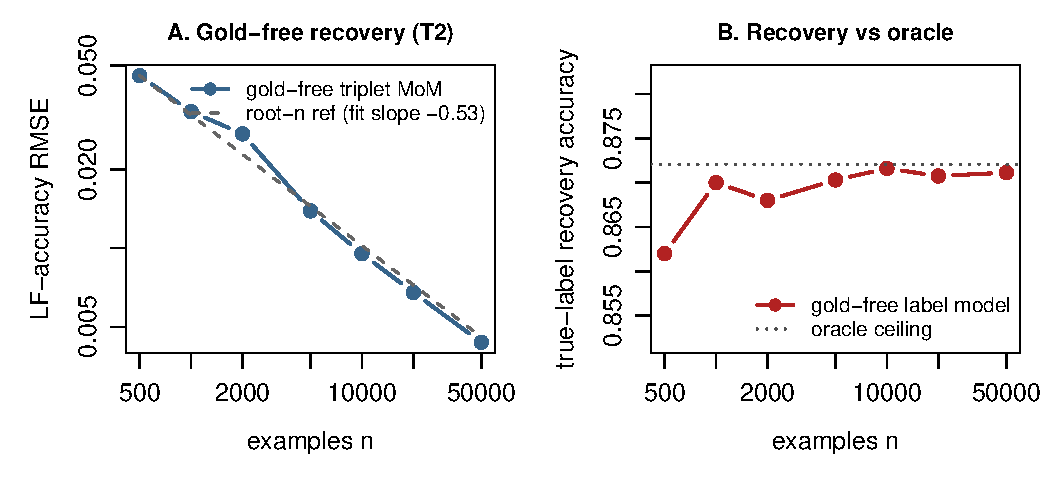
\includegraphics[width=0.95\linewidth]{identifiability_recovery.pdf}
\caption{Gold-free recovery under conditional independence
(\cref{thm:ci-identifiability}), $30$ replicates per setting. (A)
LF-accuracy RMSE decreases at the $n^{-1/2}$ rate (fitted log--log
slope $-0.53$). (B) True-label recovery accuracy converges to the
oracle ceiling (dashed). No gold-labeled examples are used.}
\label{fig:identifiability}
\end{figure}

\subsection{Agreement consistency (\cref{thm:agreement-consistency})}

We generate five conditionally independent LFs ($\bm{\alpha} =
(0.80, 0.74, 0.71, 0.86, 0.69)$, coverage $0.75$, $\pi = 0.5$) and
measure the residual between the model-implied and the empirical
pairwise LF agreement rates. At $n = 500{,}000$ the gold-free fit has
maximum absolute agreement residual $3.0 \times 10^{-3}$ across all
LF pairs (median $1.9 \times 10^{-4}$); the oracle fit, which uses
the true accuracies, has maximum residual $1.9 \times 10^{-3}$. The
small residual is Monte-Carlo noise, not structural error: over a
finite-$n$ sweep ($25$ replicates per setting) the median absolute
residual falls monotonically from $9.3 \times 10^{-3}$ at $n = 500$
to $7.1 \times 10^{-4}$ at $n = 100{,}000$, tracking the $n^{-1/2}$
sampling rate. The fitted label model reproduces the empirical
pairwise agreement rates, confirming \cref{thm:agreement-consistency}.
The practical consequence stands: a model can match every observed
agreement rate and still carry biased accuracies, so an agreement-fit
check cannot diagnose accuracy bias.

\subsection{Gold-set sample complexity (\cref{thm:goldset})}

We generate eight LFs with modest accuracy margins ($\bm{\alpha} =
(0.72, 0.70, 0.71, 0.69, 0.73, 0.68, 0.80, 0.78)$, coverage $0.8$,
$\pi = 0.5$), with three dependent pairs $(1,2)$, $(3,4)$, $(5,6)$
sharing latent factors and LFs $7, 8$ left as independent anchors.

\paragraph{Dependence biases the gold-free model.} With independent
LFs the gold-free triplet estimator has accuracy RMSE $0.0058$. With
dependence at $\rho = 0.5$ the RMSE rises to $0.096$, a
sixteen-fold increase. The agreement-matrix rank-deficit diagnostic,
which compares the centered pairwise agreement matrix to its
best rank-one fit $\bm{a}\bm{a}^\top$, reports effective deficit $0$
for the independent ensemble and $6$ for the dependent ensemble: LF
dependence destroys identifying directions, exactly the rank deficit
$r$ of \cref{thm:goldset}.

\paragraph{Gold labels restore identifiability.} Sweeping the
gold-set size $m_{\mathrm{gold}}$ at fixed dependence $\rho = 0.5$
($40$ replicates per setting), the gold-augmented label model's
accuracy RMSE falls monotonically from $0.096$ (gold-free) to
$0.048$ at $m_{\mathrm{gold}} = 100$, $0.036$ at $200$, and $0.017$
at $800$ (\Cref{fig:goldset}A). True-label recovery accuracy rises
from $0.825$ to $0.878$ over the same range. A modest gold set buys
back the identifiability that LF dependence removes.

\paragraph{Sample complexity scales as $1/\mathrm{gap}^2$.} We hold
the dependence structure fixed and vary the LF accuracy margin
$\mathrm{gap}$, requiring the gold-set accuracy estimate to reach a
precision proportional to $\mathrm{gap}$ (the separation between the
near-degenerate solutions). The number of gold-labeled examples
needed falls from $140$ at $\mathrm{gap} = 0.10$ to $70$ at $0.14$,
$35$ at $0.20$, $18$ at $0.28$, and $8$ at $0.40$
(\Cref{fig:goldset}B). The log--log slope of $m_{\mathrm{gold}}$
against $\mathrm{gap}$ is $-2.04$, matching the $1/\mathrm{gap}^2$
scaling of the bound \eqref{eq:goldset-bound} in
\cref{thm:goldset}. Strong, confident LF ensembles are cheap to
identify; ensembles of near-random LFs need quadratically more gold
data.

\begin{figure}[t]
\centering
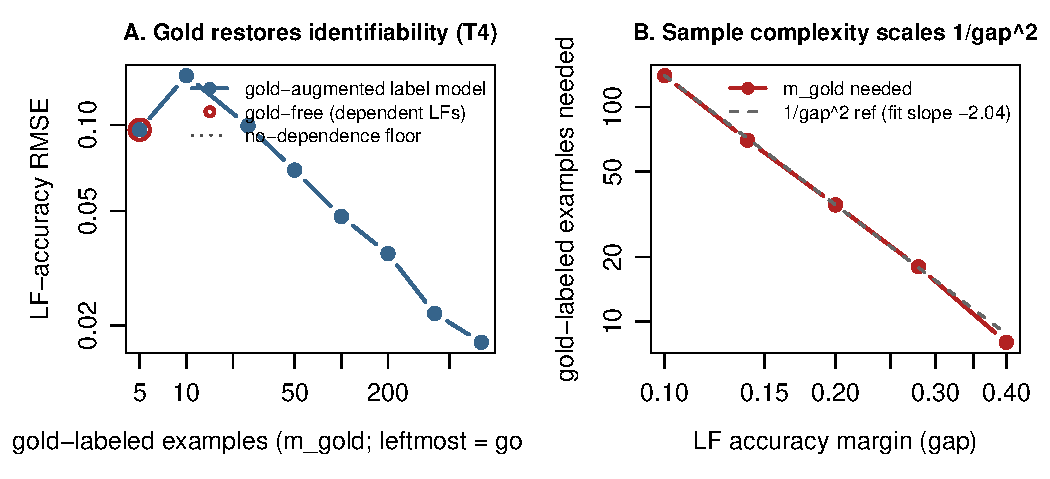
\includegraphics[width=0.95\linewidth]{goldset_complexity.pdf}
\caption{Gold-set sample complexity under LF dependence
(\cref{thm:goldset}). (A) At fixed dependence $\rho = 0.5$, the
gold-augmented label model's accuracy RMSE falls from the gold-free
value (open circle) toward the no-dependence floor (dashed) as the
gold set grows. (B) The number of gold-labeled examples needed
scales as $1/\mathrm{gap}^2$ in the LF accuracy margin (fitted
log--log slope $-2.04$).}
\label{fig:goldset}
\end{figure}

\paragraph{On the rank deficit.} The agreement-residual diagnostic and
the relative residual of the rank-one fit both grow monotonically with
the dependence strength $\rho$ (relative residual $0.08$ at $\rho =
0.1$, rising to $0.47$ at $\rho = 0.6$), and the gold-free bias tracks
them. The diagnostic reports an effective deficit of $6$ for the three
dependent pairs, which is the residual-matrix rank $2 d_{\mathrm{free}}$
of \cref{rmk:r-definition}; the parameter-degeneracy dimension is
$d_{\mathrm{free}} = 3$, one per dependent pair. The simple
gold-augmented estimator used here is the \emph{direct-marginal}
estimator: it re-measures all $m$ marginal LF accuracies from gold and
discards the agreement moments, so its cost is governed by the
$\mathrm{gap}$ term and is independent of $r$ (a union over $m$ LFs
gives $\Theta(\log m/\mathrm{gap}^2)$, with $m = 8$ fixed here). The
linear-in-$r$ rate $\Theta(r/\mathrm{gap}^2)$ of \cref{thm:goldset}
pertains instead to the hybrid estimator that uses the agreement
moments for the identified subspace and gold only for the $r$
degenerate directions; this study fixes the dependence structure and
sweeps $\mathrm{gap}$, so it isolates the $1/\mathrm{gap}^2$ factor
common to both estimators and does not exercise the $r$-channel (an
$r$-sweep with the hybrid estimator is deferred to the longer manuscript
\citep{towell2026weaksupcoarseningextended}). The two checkable
predictions of \cref{thm:goldset}, that gold labels restore
identifiability and that the cost scales as $1/\mathrm{gap}^2$, both
hold.

Direct comparison with the Snorkel and FlyingSquid implementations
on the WRENCH benchmark \citep{ratner2017snorkel,fu2020fast,
zhang2021wrench} is left to the longer
manuscript~\citep{towell2026weaksupcoarseningextended}; the framework applies
to the LF-vote matrix that is the input of each method without
modification.

\section{Discussion}
\label{sec:discussion}

This paper is one application of the masked-cause coarsening
framework of \citet{towell2026masked}; the shared identifiability
vocabulary is what the series argues for, and each application
contributes a domain-specific construction (here, the glass-ceiling
symmetry and the gold-set sample-complexity bound).

\subsection{Relation to prior work on label-model identifiability}

Label-model identifiability has a deep prior literature, and an
honest account places this paper's contribution against it.

\paragraph{Dawid--Skene is the ancestor.} \citet{dawid1979maximum}
posed and solved the core problem: estimate per-rater error rates and
a class prior, by maximum likelihood via EM, from rater votes alone.
Every label model in programmatic weak supervision, and the
masked-cause statement of it in this paper, is a descendant of that
work. The EM solver of Dawid--Skene is the maximum-likelihood solver
for the coarsened likelihood \eqref{eq:bg-c1c2c3}; the framework here
does not replace it, it gives it an identifiability vocabulary.

\paragraph{Moment-based identifiability is established.} Data
programming \citep{ratner2016data} showed that LF accuracies are
recoverable from agreement statistics under conditional independence;
the triplet method of \citet{fu2020fast} made the recovery a
closed form in third-order agreement moments; the multi-task
extension \citep{ratner2019training,ratner2020training} handled
structured dependence with a known dependency graph;
\citet{bach2017learning} showed the dependency structure can
sometimes be learned, but only under restrictive conditions.
\Cref{thm:ci-identifiability} is a re-derivation of this body of
results, not a new identifiability claim. The crowdsourcing
literature \citep{karger2011iterative,zhang2016spectral} solved the
same estimation problem for human annotators; the spectral and
tensor-decomposition tools \citep{anandkumar2014tensor} use the
same low-rank moment structure that underlies the masked-cause
augmented-matrix rank condition (\cref{thm:bg-id}). The Snorkel
ecosystem \citep{ratner2018snorkelmetal,bach2019snorkeldrybell,
sala2019multiresolution,zhang2022survey} has expanded weak
supervision to multi-task, deployment, sequential, and interactive
\citep{boecking2021interactive} settings; the masked-cause framework
applies to each, because all share the LF-vote-matrix input.

\paragraph{What this paper adds.} The contribution is narrower than
``label-model identifiability'' and is fourfold. (i) The masked-cause
unification: LF votes are a candidate-set coarsening, abstention is a
non-informative candidate set, a confident vote is a narrowed one,
and gold labels are singletons. This places weak supervision in the
same frame as the other applications of the masked-cause framework
\citep{towell2026masked}. (ii) The C1--C2--C3 classification of LF
ensembles: the three coarsening-at-random conditions become checkable
statements about an LF set (support, label-only error dependence,
parameter separation). (iii) The explicit glass-ceiling construction:
the accuracy-complement symmetry of \cref{thm:glass-ceiling} is a
precise statement, with an exact label-flip witness, of why gold-free
estimation cannot orient the model. (iv) The gold-set
sample-complexity theorem for the dependent case
(\cref{thm:goldset}): prior work establishes the conditionally
independent corner ($r = 0$); the $\Theta(r / \mathrm{gap}^2)$ bound
for total model recovery extends it to the correlated ensembles that
practice produces, and the $1/\mathrm{gap}^2$ scaling is confirmed in
simulation. We do not
claim to invent label-model identifiability; we claim a unifying
frame, a classification, and a sample-complexity result for the
dependent case.

\subsection{What the framework does \emph{not} address}

\begin{itemize}
\item \textbf{Multiclass and structured outputs.} The development is
  binary. The masked-cause framework extends to a categorical latent
  cause directly, and Dawid--Skene is natively multiclass; the
  C1--C2--C3 statements and the rank arguments carry over, but we did
  not write out the multiclass theorems here.

\item \textbf{Unknown dependency structure.} \Cref{thm:goldset}
  assumes the rank deficit $r$ is a property of the ensemble, but
  $r$ is itself estimated. Recovering the dependency graph from data,
  rather than assuming it as in \citet{ratner2019training}, is a
  harder problem the framework does not solve.

\item \textbf{Abstention that depends on the label.} We model
  coverage $\beta_j$ as independent of $Y$. An LF that abstains
  preferentially on one class is a label-dependent coarsening, a C2
  violation the present analysis does not cover; the C2-relaxation
  results of \citet{towell2026mdrelax} are the natural tool.

\item \textbf{The downstream model.} The framework analyzes the label
  model. Whether the probabilistic training labels it emits yield a
  good downstream classifier is a separate generalization question,
  governed by the end-to-end analysis of \citet{ratner2016data}.

\item \textbf{Adversarial or systematically wrong LFs.} C1 fails when
  an LF is confidently wrong beyond the modeled noise. Such LFs need
  detection and removal, which the framework flags as a C1 violation
  but does not itself perform.
\end{itemize}

\subsection{Broader implications}

The framework shifts the question a weak-supervision practitioner
asks from ``which label model should I use?'' to ``which
coarsening-at-random conditions does my LF ensemble satisfy?'' If the
LFs are conditionally independent and better than random, the
ensemble is on the identifiable side of the boundary and a gold-free
pipeline is sound (\cref{thm:ci-identifiability}). If the LFs are
correlated, the ensemble is rank-deficient and gold labels are
required, with a budget set by the rank deficit and the accuracy
margin (\cref{thm:goldset}). If an LF is confidently wrong, C1 fails
and no aggregation rescues it. This is the same assumption-specific
reasoning previously brought to other masked-cause applications in
the framework series \citep{towell2026masked}: recognizing the
common masked-cause structure lets one identifiability apparatus
serve measurement problems that look unrelated on the surface. The
framework series collectively argues that the candidate-set
abstraction is a general tool for any inference problem in which
observations partially-determine a latent cause.

\section{Conclusion}
\label{sec:conclusion}

Programmatic weak supervision fits a label model from noisy labeling
functions, ideally without gold-labeled data. The central question,
when the true labels can be recovered from LF votes alone, is the
masked-cause identifiability problem from reliability statistics: the
true label is the latent cause, the labels consistent with the LF
votes are the candidate set, an LF abstention is a non-informative
candidate set, a confident vote is a narrowed one, and a gold-labeled
example is a singleton candidate set. We proved (i) a glass-ceiling
theorem, with an exact accuracy-complement symmetry, showing that
gold-free estimation cannot orient the label model without a
structural assumption; (ii) an identifiability theorem recovering the
Dawid--Skene, data-programming, and triplet-method result as a
masked-cause statement under conditional independence; (iii) an
agreement-consistency theorem showing the fitted model reproduces
empirical pairwise LF agreement rates exactly at an interior MLE; and
(iv) a gold-set sample-complexity bound, $\Theta(r / \mathrm{gap}^2)$
for total (L2) model recovery in the parameter-degeneracy dimension
induced by LF dependence and the accuracy margin, for restoring
identifiability when LFs are correlated. A base-R
simulation confirmed all four: the symmetry is exact, gold-free
recovery under conditional independence reaches the oracle ceiling,
the agreement residual is Monte-Carlo noise, and the gold-set
requirement scales as $1/\mathrm{gap}^2$ with fitted log--log slope
$-2.04$.

Dawid--Skene (1979) is the clear ancestor of the label model, and
moment-based identifiability for conditionally independent LFs is
established prior work; the contribution here is the masked-cause
unification, the C1--C2--C3 classification of LF ensembles, the
explicit glass-ceiling construction, and the sample-complexity result
for the dependent case. The framework gives a practitioner a
diagnostic: a gold-free pipeline is sound when the LF ensemble
satisfies the coarsening-at-random conditions, and the gold budget
needed otherwise is set by the rank deficit and the accuracy margin.

The principal open extensions are the multiclass and structured-output
theorems, data-driven recovery of the LF dependency graph,
label-dependent abstention via the C2-relaxation results of
\citet{towell2026mdrelax}, and a head-to-head study against the
Snorkel and FlyingSquid implementations on the WRENCH benchmark.
Each is a natural follow-up.


\bibliographystyle{plainnat}
\bibliography{refs}

\end{document}
